% !TEX root = ../../../main.tex
% 所属：第四部分：Fourier 分析 / 第7章：Dirichlet定理
% 节：7.3 Dirichlet定理的证明
% 正文按原文件顺序保存；由 ../chapter7.tex 调用。
\section{Dirichlet定理的证明}

首先处理复对数。

\begin{definition}
	对 $\abs z<1$，定义
\begin{equation}\label{eq:log-one-definition}
	\log_1\left(\frac1{1-z}\right)
	=\sum_{k=1}^{\infty}\frac{z^k}{k}.
\end{equation}
\end{definition}
若令
\[
w=\frac1{1-z}=x+iy,
\qquad
z=\frac{w-1}{w},
\]
则
\[
\abs z<1
\iff \abs{w-1}<\abs w
\iff (x-1)^2+y^2<x^2+y^2
\iff x>\frac12.
\]
因此，$\log_1w$ 在半平面 $\Re w>1/2$ 上有定义；当
$w>1/2$ 为实数时，它与通常的实对数一致。

\begin{proposition}\label{prop:log-one-properties}
	函数 $\log_1$ 具有下列性质：
	\begin{enumerate}[label=\textup{(\roman*)}]
		\item 若 $\abs z<1$，则
		\[
		e^{\log_1\left(\frac1{1-z}\right)}=\frac1{1-z}.
		\]
		\item 若 $\abs z<1$，则
		\[
		\log_1\left(\frac1{1-z}\right)=z+E_1(z),
		\]
		且当 $\abs z\leq1/2$ 时，
		$\abs{E_1(z)}\leq\abs z^2$。
		\item 若 $\abs z<1/2$，则
		\[
		\abs{\log_1\left(\frac1{1-z}\right)}\leq2\abs z.
		\]
	\end{enumerate}
\end{proposition}

\begin{proof}
	令 $z=re^{i\theta}$，其中 $0\leq r<1$，并记
	\[
	F(r)=(1-re^{i\theta})
	\exp\left(\sum_{k=1}^{\infty}\frac{(re^{i\theta})^k}{k}\right).
	\]
	逐项求导可得
	\[
	F'(r)=0.
	\]
	又 $F(0)=1$，故 $F(r)=1$，这就证明了 \textup{(i)}。

	由定义，
	\[
	E_1(z)=\sum_{k=2}^{\infty}\frac{z^k}{k}.
	\]
	当 $\abs z\leq1/2$ 时，
	\[
	\abs{E_1(z)}
	\leq\frac{\abs z^2}{2}\sum_{j=0}^{\infty}\abs z^j
	\leq\abs z^2,
	\]
	从而得到 \textup{(ii)}。最后，
	\[
	\abs{\log_1\left(\frac1{1-z}\right)}
	\leq\abs z+\abs{E_1(z)}
	\leq2\abs z,
	\]
	故 \textup{(iii)} 成立。
\end{proof}

\begin{proposition}\label{prop:absolute-convergence-infinite-product}
	若 $\sum\limits_{n=1}^{\infty}\abs{a_n}$ 收敛，且对任意 $n$ 都有
	$a_n\neq1$，则无穷乘积
	\[
	\prod_{n=1}^{\infty}\frac1{1-a_n}
	\]
	收敛且不为零。
\end{proposition}

\begin{proof}
	对充分大的 $n$，有 $\abs{a_n}<1/2$。去掉有限项不影响结论，
	故不妨设这一不等式对所有 $n$ 成立。由命题
	\ref{prop:log-one-properties}，
	\[
	\abs{\log_1\left(\frac1{1-a_n}\right)}
	\leq2\abs{a_n}.
	\]
	因此级数
	\[
	\sum_{n=1}^{\infty}
	\log_1\left(\frac1{1-a_n}\right)
	\]
	绝对收敛，设其和为 $A$。于是
	\[
	\prod_{n=1}^{N}\frac1{1-a_n}
	=\exp\left(
	\sum_{n=1}^{N}\log_1\left(\frac1{1-a_n}\right)
	\right)
	\longrightarrow e^A\neq0.
	\]
\end{proof}

现在严格证明定理 \ref{thm:dirichlet-L-euler-product}。

\begin{proof}[定理 \ref{thm:dirichlet-L-euler-product}的证明]
为简化记号，令
\[
L=L(s,\chi),
\qquad
S_N=\sum_{n\leq N}\frac{\chi(n)}{n^s},
\qquad
\Pi_N=\prod_{p\leq N}\frac1{1-\chi(p)p^{-s}}.
\]
由命题 \ref{prop:absolute-convergence-infinite-product}，当 $s>1$ 时
无穷乘积
\[
\Pi=\lim_{N\to\infty}\Pi_N
=\prod_p\frac1{1-\chi(p)p^{-s}}
\]
收敛且不为零。事实上，若 $p_n$ 是第 $n$ 个素数，并令
$a_n=\chi(p_n)p_n^{-s}$，则
\[
\sum_n\abs{a_n}\leq\sum_{n=1}^{\infty}\frac1{n^s}<\infty.
\]

再定义有限乘积
\[
\Pi_{N,M}
=\prod_{p\leq N}
\left(1+\frac{\chi(p)}{p^s}+\cdots
+\frac{\chi(p^M)}{p^{Ms}}\right).
\]
固定 $\varepsilon>0$。先取充分大的 $N$，使得
\[
\abs{S_N-L}<\varepsilon,
\qquad
\abs{\Pi_N-\Pi}<\varepsilon,
\qquad
\sum_{n>N}\frac1{n^s}<\varepsilon.
\]
再取充分大的 $M$。由算术基本定理及 $\chi$ 的完全可乘性，
$\Pi_{N,M}$ 的展开式包含 $S_N$ 的全部项，其余项所对应的整数
均大于 $N$，故
\[
\abs{S_N-\Pi_{N,M}}<\varepsilon.
\]
另一方面，有限个几何级数分别收敛，所以还可令
\[
\abs{\Pi_{N,M}-\Pi_N}<\varepsilon.
\]
因此
\[
\abs{L-\Pi}
\leq\abs{L-S_N}
+\abs{S_N-\Pi_{N,M}}
+\abs{\Pi_{N,M}-\Pi_N}
+\abs{\Pi_N-\Pi}
<4\varepsilon.
\]
由 $\varepsilon$ 的任意性，得到
\[
L(s,\chi)=\prod_p\frac1{1-\chi(p)p^{-s}},
\qquad s>1.
\]
\end{proof}
\newpage
\begin{proposition}\label{prop:principal-character-L-function}
	设 $\chi_0$ 是模 $q$ 的平凡 Dirichlet 特征，且
	\[
	q=p_1^{a_1}\cdots p_N^{a_N}
	\]
	是 $q$ 的素因子分解，则
	\[
	L(s,\chi_0)
	=\left(1-\frac1{p_1^s}\right)
	\cdots
	\left(1-\frac1{p_N^s}\right)\zeta(s).
	\]
	因此，当 $s\to1^+$ 时，$L(s,\chi_0)\to\infty$。
\end{proposition}

\begin{proof}
	比较 $L(s,\chi_0)$ 与 $\zeta(s)$ 的 Euler 乘积，便有
	\[
	L(s,\chi_0)
	=\prod_{p\nmid q}\frac1{1-p^{-s}}
	=\zeta(s)\prod_{p\mid q}(1-p^{-s}).
	\]
	当 $s\to1^+$ 时，右边的有限乘积趋于一个正数，而
	$\zeta(s)\to\infty$，故结论成立。
\end{proof}

\begin{proposition}\label{prop:nonprincipal-L-properties}
	若 $\chi$ 是非平凡的 Dirichlet 特征，则当 $s>0$ 时，级数
	\[
	\sum_{n=1}^{\infty}\frac{\chi(n)}{n^s}
	\]
	收敛，记其和为 $L(s,\chi)$。并且：
	\begin{enumerate}[label=\textup{(\roman*)}]
		\item $L(s,\chi)$ 在 $0<s<\infty$ 上连续可微；
		\item 当 $s\to\infty$ 时，存在常数 $c,c'>0$，使得
		\[
		L(s,\chi)=1+O(e^{-cs}),
		\qquad
		L'(s,\chi)=O(e^{-c's}).
		\]
	\end{enumerate}
\end{proposition}

先给出非平凡 Dirichlet 特征的一个关键消失性结论。

\begin{lemma}\label{lem:dirichlet-character-partial-sums}
	若 $\chi$ 是模 $q$ 的非平凡 Dirichlet 特征，则对任意正整数
	$k$，有
	\[
	\abs{\sum_{n=1}^{k}\chi(n)}\leq q.
	\]
\end{lemma}

\begin{proof}
	首先证明
	\[
	\sum_{n=1}^{q}\chi(n)=0.
	\]
	记左边为 $S$。对任意 $a\in\Z^*(q)$，乘法 $n\mapsto an$
	置换模 $q$ 的剩余类，因此
	\[
	\chi(a)S
	=\sum_{n=1}^{q}\chi(a)\chi(n)
	=\sum_{n=1}^{q}\chi(an)
	=S.
	\]
	由于 $\chi$ 非平凡，可取 $a$ 使 $\chi(a)\neq1$，故 $S=0$。

	写成 $k=mq+b$，其中 $0\leq b<q$。利用 $\chi$ 的周期性，
	前 $m$ 个完整周期的和均为零，所以
	\[
	\sum_{n=1}^{k}\chi(n)
	=\sum_{n=mq+1}^{mq+b}\chi(n).
	\]
	右边至多有 $q$ 项，且 $\abs{\chi(n)}\leq1$，结论得证。
\end{proof}

\begin{proof}[命题 \ref{prop:nonprincipal-L-properties} 的证明]
	记
	\[
	s_k=\sum_{n=1}^{k}\chi(n),
	\qquad s_0=0.
	\]
	当 $s>1$ 时，$L(s,\chi)$ 的级数绝对收敛。对有限和作Abel变换，
	得到
	\[
	\begin{aligned}
	\sum_{k=1}^{N}\frac{\chi(k)}{k^s}
	&=\sum_{k=1}^{N}\frac{s_k-s_{k-1}}{k^s}\\
	&=\sum_{k=1}^{N-1}s_k
	\left(\frac1{k^s}-\frac1{(k+1)^s}\right)
	+\frac{s_N}{N^s}.
	\end{aligned}
	\]
	令
	\[
	f_k(s)=s_k\left(\frac1{k^s}-\frac1{(k+1)^s}\right).
	\]
	由引理 \ref{lem:dirichlet-character-partial-sums} 及中值定理，
	\[
	\abs{f_k(s)}\leq qs k^{-s-1}.
	\]
	因此 $\sum\limits_k f_k(s)$ 在 $s>0$ 的每个紧区间上一致收敛，且
$s_NN^{-s}\to0$。这既把 $L(s,\chi)$ 延拓到 $s>0$，也证明了
	其连续性。

	逐项求导时出现的级数为
	\[
	-\sum_{n=1}^{\infty}(\log n)\frac{\chi(n)}{n^s}.
	\]
	再次作Abel变换，其相应级数可以写为
	\[
	\sum_{k=1}^{\infty}s_k
	\left[-\frac{\log k}{k^s}
	+\frac{\log(k+1)}{(k+1)^s}\right].
	\]
	由中值定理和 $\abs{s_k}\leq q$，该级数同样在 $s>0$ 的
	每个紧区间上一致收敛，故 $L(s,\chi)$ 在 $s>0$ 上连续可微。

	最后，当 $s$ 充分大时，
	\[
	\abs{L(s,\chi)-1}
	\leq\sum_{n=2}^{\infty}\frac1{n^s}
	=2^{-s}+\int_{3}^{\infty}x^{-s}\dd x=O(2^{-s}),
	\]
	而
	\[
	\abs{L'(s,\chi)}
	\leq\sum_{n=2}^{\infty}\frac{\log n}{n^s}
	=O(e^{-c's})
	\]
	对某个 $c'>0$ 成立。取 $c=\log2$，即得 \textup{(ii)}。
\end{proof}

现在可以定义 $L$ 函数的另一种对数。

\begin{definition}
	若 $\chi$ 是非平凡的
Dirichlet 特征，对 $s>1$ 定义
\begin{equation}\label{eq:log-two-L-definition}
	\log_2L(s,\chi)
	=-\int_s^{\infty}\frac{L'(t,\chi)}{L(t,\chi)}\dd t.
\end{equation}
\end{definition}
由 Euler 乘积及命题
\ref{prop:absolute-convergence-infinite-product}，$L(t,\chi)\neq0$
对所有 $t>1$ 成立。再由命题
\ref{prop:nonprincipal-L-properties}，
\[
\frac{L'(t,\chi)}{L(t,\chi)}=O(e^{-ct})
\]
对充分大的 $t$ 成立，因此上述积分收敛。

\begin{proposition}\label{prop:two-logarithms-for-L}
	若 $s>1$，则
	\[
	e^{\log_2L(s,\chi)}=L(s,\chi).
	\]
	进而
	\[
	\log_2L(s,\chi)
	=\sum_p\log_1\left(
	\frac1{1-\chi(p)p^{-s}}
	\right).
	\]
\end{proposition}

\begin{proof}
	对 $e^{-\log_2L(s,\chi)}L(s,\chi)$ 关于 $s$ 求导，由
式 \eqref{eq:log-two-L-definition} 可知导数为零。因此它是常数。
当 $s\to\infty$ 时，$L(s,\chi)\to1$ 且
$\log_2L(s,\chi)\to0$，故这个常数等于 $1$，从而
\[
	e^{\log_2L(s,\chi)}=L(s,\chi).
\]

	另一方面，由命题 \ref{prop:log-one-properties} 与 Euler 乘积，
	\[
	\begin{aligned}
	\exp\left\{
	\sum_p\log_1\left(
	\frac1{1-\chi(p)p^{-s}}
	\right)
	\right\}
	&=\prod_p
	\exp\left\{
	\log_1\left(
	\frac1{1-\chi(p)p^{-s}}
	\right)
	\right\}\\
	&=\prod_p\frac1{1-\chi(p)p^{-s}}
	=L(s,\chi).
	\end{aligned}
	\]
	所以对每个 $s>1$，存在整数 $M(s)$，使得
	\[
	\log_2L(s,\chi)
	-\sum_p\log_1\left(
	\frac1{1-\chi(p)p^{-s}}
	\right)
	=2\pi iM(s).
	\]
	左边关于 $s$ 连续，故整数值函数 $M(s)$ 为常数。令
$s\to\infty$，可知该常数为 $0$，第二个等式得证。
\end{proof}

把上述结论合在一起，由命题 \ref{prop:log-one-properties}，
\[
\begin{aligned}
\sum_p\log_1\left(
\frac1{1-\chi(p)p^{-s}}
\right)
&=\sum_p\frac{\chi(p)}{p^s}
+O\left(\sum_p\frac1{p^{2s}}\right)\\
&=\sum_p\frac{\chi(p)}{p^s}+O(1).
\end{aligned}
\]
若 $\chi$ 是非平凡 Dirichlet 特征且 $L(1,\chi)\neq0$，则由
式 \eqref{eq:log-two-L-definition} 及命题
\ref{prop:nonprincipal-L-properties}，当 $s\to1^+$ 时
$\log_2L(s,\chi)$ 仍然有界。结合命题
\ref{prop:two-logarithms-for-L}，可知
\[
\sum_p\frac{\chi(p)}{p^s}
\]
保持有界，这正是定理
\ref{thm:nonprincipal-prime-character-sum-bounded} 所需的结论。
因此，为完成 Dirichlet 定理的证明，只需证明：当 $\chi$ 为
非平凡 Dirichlet 特征时，
\[
L(1,\chi)\neq0.
\]

\begin{theorem}\label{thm:dirichlet-L-nonvanishing-at-one}
	若 $\chi\neq\chi_0$，则
	\[
	L(1,\chi)\neq0.
	\]
\end{theorem}

按照 $\chi$ 是实值还是复值，将证明分为两种情形。若
$\chi(n)\in\{0,1,-1\}$ 对所有整数 $n$ 成立，则称 $\chi$ 为
实 Dirichlet 特征；否则称为复 Dirichlet 特征。

\subsection*{情形一：复 Dirichlet 特征}

这一情形使用反证法。先给出两个引理。

\begin{lemma}\label{lem:product-all-dirichlet-L-positive}
	若 $s>1$，则
	\[
	\prod_\chi L(s,\chi)\geq1,
	\]
	其中乘积取遍模 $q$ 的所有 Dirichlet 特征。特别地，这个乘积
	是实数。
\end{lemma}

\begin{proof}
	由命题 \ref{prop:two-logarithms-for-L}，当 $s>1$ 时
	\[
	L(s,\chi)
	=\exp\left[
	\sum_p\log_1\left(
	\frac1{1-\chi(p)p^{-s}}
	\right)
	\right].
	\]
	因此
	\[
	\begin{aligned}
	\prod_\chi L(s,\chi)
	&=\exp\left[
	\sum_\chi\sum_p
	\log_1\left(
	\frac1{1-\chi(p)p^{-s}}
	\right)
	\right]\\
	&=\exp\left[
	\sum_p\sum_{k=1}^{\infty}
	\frac1{k p^{ks}}
	\sum_\chi\chi(p^k)
	\right].
	\end{aligned}
	\]
	由引理 \ref{lem:dirichlet-character-multiplicativity-delta}，取
$\ell=1$，有
	\[
	\sum_\chi\chi(p^k)=\varphi(q)\delta_1(p^k).
	\]
	故
	\[
	\prod_\chi L(s,\chi)
	=\exp\left[
	\varphi(q)\sum_p\sum_{k=1}^{\infty}
	\frac{\delta_1(p^k)}{k p^{ks}}
	\right]\geq1,
	\]
	因为指数中的每一项都是非负实数。
\end{proof}

\begin{lemma}\label{lem:L-conjugation-and-near-one-bounds}
	下列结论成立：
	\begin{enumerate}[label=\textup{(\roman*)}]
		\item 若 $L(1,\chi)=0$，则 $L(1,\overline\chi)=0$；
		\item 若 $\chi$ 非平凡且 $L(1,\chi)=0$，则当
		$1\leq s\leq2$ 时
		\[
		\abs{L(s,\chi)}\leq C\abs{s-1};
		\]
		\item 对平凡特征 $\chi_0$，当 $1<s\leq2$ 时
		\[
		\abs{L(s,\chi_0)}\leq\frac{C}{\abs{s-1}}.
		\]
	\end{enumerate}
\end{lemma}

\begin{proof}
	因为 $L(s,\overline\chi)=\overline{L(s,\chi)}$，故
\textup{(i)} 成立。若 $\chi$ 非平凡，则由命题
\ref{prop:nonprincipal-L-properties}，$L(s,\chi)$ 在 $s>0$ 上
连续可微；若 $L(1,\chi)=0$，由平均值定理得到 \textup{(ii)}。
最后，由命题 \ref{prop:principal-character-L-function}，
	\[
	L(s,\chi_0)=\zeta(s)\prod_{p\mid q}(1-p^{-s}),
	\]
	并且 $\zeta(s)\leq1+(s-1)^{-1}$，所以 \textup{(iii)} 成立。
\end{proof}

\begin{proof}[情形一的证明]
	现在设 $\chi$是非平凡的复 Dirichlet 特征，并反设
$L(1,\chi)=0$。由引理
\ref{lem:L-conjugation-and-near-one-bounds}，也有
$L(1,\overline\chi)=0$。因为 $\chi\neq\overline\chi$，所以
\[
\prod_\psi L(s,\psi)
\]
中至少有两个因子在 $s=1$ 处为零。其余非平凡特征对应的
$L$ 函数在 $s=1$ 附近有界，而平凡特征对应的因子至多以
$\abs{s-1}^{-1}$ 的速度增长。因此，当 $s\to1^+$ 时
	\[
	\prod_\psi L(s,\psi)\longrightarrow0,
	\]
	这与引理 \ref{lem:product-all-dirichlet-L-positive} 中该乘积恒不小于
$1$ 矛盾。故复特征情形下 $L(1,\chi)\neq0$。

\end{proof}
\subsection*{情形二：实 Dirichlet 特征}

这里使用求和与积分比较以及双曲求和。先做一些准备工作。

\begin{proposition}\label{prop:harmonic-sum-asymptotic}
	对正整数 $N$，有
	\begin{enumerate}[label=\textup{(\roman*)}]
		\item
		\[
		\sum_{1\leq n\leq N}\frac1n
		=\int_1^N\frac{\dd x}{x}+O(1)
		=\log N+O(1);
		\]
		\item 存在实数 $\gamma$，使得
		\[
		\sum_{1\leq n\leq N}\frac1n
		=\log N+\gamma+O\left(\frac1N\right).
		\]
	\end{enumerate}
\end{proposition}

\begin{proof}
	第一式由积分比较立即得到。为证明第二式，令
	\[
	\gamma_n=\frac1n-\int_n^{n+1}\frac{\dd x}{x}.
	\]
	由于 $x^{-1}$ 单调递减，
	\[
	0\leq\gamma_n
	\leq\frac1n-\frac1{n+1}
	\leq\frac1{n^2}.
	\]
	故 $\sum\limits_{n=1}^{\infty}\gamma_n$ 收敛，记其和为 $\gamma$。并且
	\[
	\sum_{n=N+1}^{\infty}\gamma_n
	\leq\sum_{n=N+1}^{\infty}\frac1{n^2}
	=O\left(\frac1N\right).
	\]
	于是
	\[
	\begin{aligned}
	\sum_{n=1}^{N}\frac1n-\int_1^N\frac{\dd x}{x}
	&=\gamma-\sum_{n=N+1}^{\infty}\gamma_n
	+\int_N^{N+1}\frac{\dd x}{x}\\
	&=\gamma+O\left(\frac1N\right).
	\end{aligned}
	\]
\end{proof}

\begin{proposition}\label{prop:square-root-sum-asymptotic}
	对正整数 $N$，存在常数 $c$，使得
	\[
	\sum_{1\leq n\leq N}\frac1{\sqrt n}
	=\int_1^N\frac{\dd x}{\sqrt x}+c
	+O\left(N^{-1/2}\right)
	=2\sqrt N+c+O\left(N^{-1/2}\right).
	\]
\end{proposition}

\begin{proof}
	证明与命题 \ref{prop:harmonic-sum-asymptotic} 相同。只需注意由
中值定理，
	\[
	\abs{\frac1{\sqrt n}-\frac1{\sqrt{n+1}}}
	\leq\frac{C}{n^{3/2}},
	\]
	而 $\sum n^{-3/2}$ 收敛。
\end{proof}
\subsection*{双曲求和}
若 $F$ 是定义在正整数对上的函数，记
\[
S_N=\sum_{mn\leq N}F(m,n).
\]
同一个和可以用下列三种方式计算：
\begin{enumerate}[label=\textup{(\alph*)}]
	\item 沿双曲线分层：
	\[
	S_N=\sum_{1\leq k\leq N}\;
	\sum_{mn=k}F(m,n);
	\]
	\item 垂直求和：
	\[
	S_N=\sum_{1\leq m\leq N}\;
	\sum_{1\leq n\leq N/m}F(m,n);
	\]
	\item 水平求和：
	\[
	S_N=\sum_{1\leq n\leq N}\;
	\sum_{1\leq m\leq N/n}F(m,n).
	\]
\end{enumerate}
\begin{center}
	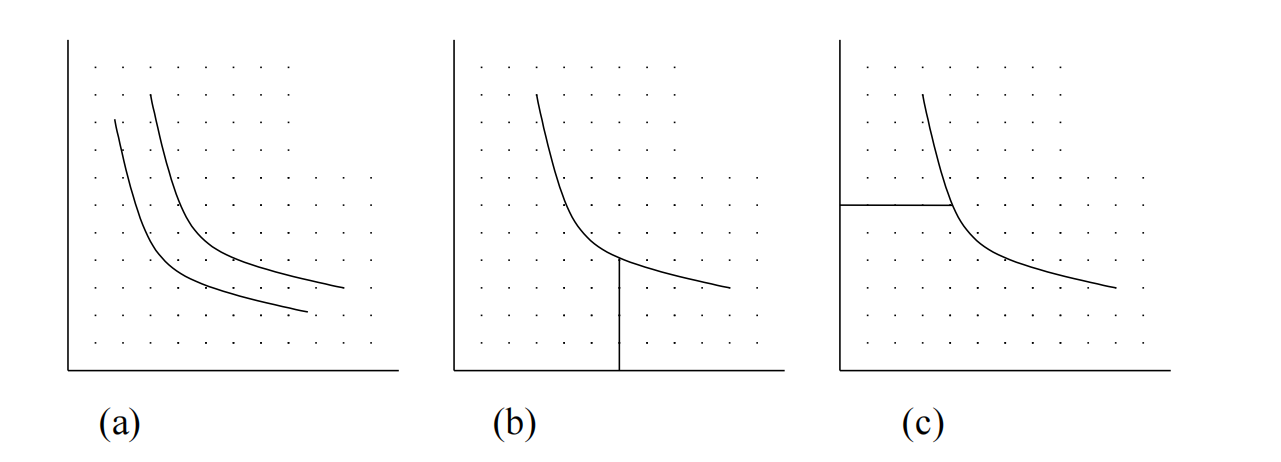
\includegraphics[width=0.9\linewidth]{figure/P4/双曲}
\end{center}

下面把双曲求和用于实 Dirichlet 特征。设 $\chi$ 是非平凡的实
Dirichlet 特征，令
\[
F(m,n)=\frac{\chi(n)}{\sqrt{mn}},
\qquad
S_N=\sum_{mn\leq N}F(m,n).
\]

\begin{proposition}\label{prop:hyperbola-sum-two-estimates}
	存在常数 $c>0$，使得
	\begin{enumerate}[label=\textup{(\roman*)}]
		\item $S_N\geq c\log N$；
		\item
		\[
		S_N=2\sqrt N\,L(1,\chi)+O(1).
		\]
	\end{enumerate}
\end{proposition}

若反设 $L(1,\chi)=0$，则 \textup{(ii)} 给出 $S_N=O(1)$，与
\textup{(i)} 矛盾。因此该命题将完成实特征情形的证明。

首先沿双曲线求和：
\[
\sum_{mn=k}\frac{\chi(n)}{\sqrt{mn}}
=\frac1{\sqrt k}\sum_{n\mid k}\chi(n).
\]

\begin{lemma}\label{lem:real-character-divisor-sum-positive}
	若 $\chi$ 是实 Dirichlet 特征，则对任意正整数 $k$，
	\[
	\sum_{n\mid k}\chi(n)\geq0.
	\]
	若 $k=\ell^2$ 是完全平方数，则
	\[
	\sum_{n\mid k}\chi(n)\geq1.
	\]
\end{lemma}

\begin{proof}
	先设 $k=p^a$。由完全可乘性，
	\[
	\sum_{n\mid p^a}\chi(n)
	=1+\chi(p)+\chi(p)^2+\cdots+\chi(p)^a.
	\]
	由于 $\chi(p)\in\{0,1,-1\}$，右边等于
	\[
	\begin{cases}
		a+1,&\chi(p)=1,\\
		1,&\chi(p)=-1\text{ 且 }a\text{ 为偶数},\\
		0,&\chi(p)=-1\text{ 且 }a\text{ 为奇数},\\
		1,&\chi(p)=0.
	\end{cases}
	\]
	一般地，若 $k=p_1^{a_1}\cdots p_r^{a_r}$，则
	\[
	\sum_{n\mid k}\chi(n)
	=\prod_{j=1}^{r}
	\left(1+\chi(p_j)+\chi(p_j)^2+\cdots+\chi(p_j)^{a_j}\right).
	\]
	每个因子均非负；若 $k$ 是平方数，则每个 $a_j$ 都是偶数，
每个因子至少为 $1$。
\end{proof}

由此，
\[
S_N
=\sum_{k\leq N}\frac1{\sqrt k}\sum_{n\mid k}\chi(n)
\geq\sum_{\ell^2\leq N}\frac1\ell
\geq c\log N,
\]
其中最后一个不等式来自命题
\ref{prop:harmonic-sum-asymptotic}。这证明了命题
\ref{prop:hyperbola-sum-two-estimates} 的 \textup{(i)}。

为了证明 \textup{(ii)}，将区域 $mn\leq N$ 分为
\[
\begin{aligned}
I&=\{1\leq m<\sqrt N,\ \sqrt N<n\leq N/m\},\\
II&=\{1\leq m\leq\sqrt N,\ 1\leq n\leq\sqrt N\},\\
III&=\{\sqrt N<m\leq N/n,\ 1\leq n\leq\sqrt N\}.
\end{aligned}
\]

\begin{center}
		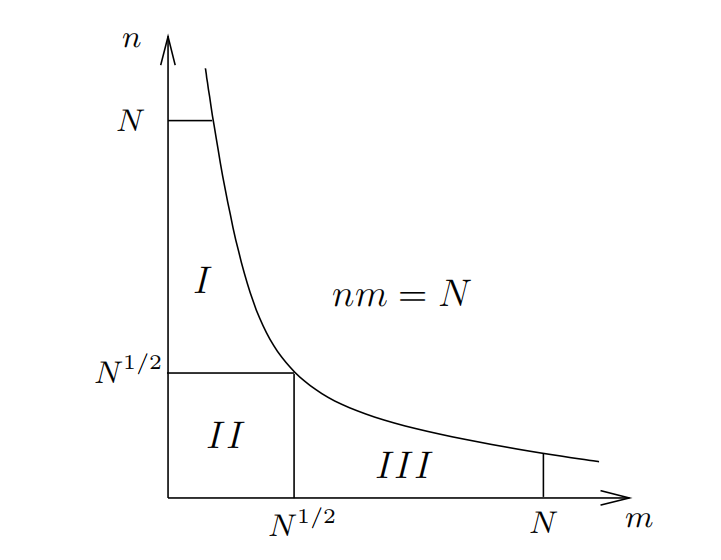
\includegraphics[width=0.7\linewidth]{figure/P4/1,2,3}
\end{center}

分别记这些区域上的和为 $S_I,S_{II},S_{III}$。区域 $I$ 与区域
$III$ 关于 $m=n$ 对称。由于这里的被加函数未必关于 $m,n$ 对称，
在估计时写成
\[
S_N=S_I+(S_{II}+S_{III}),
\]
其中对 $S_I$ 作垂直求和，对 $S_{II}+S_{III}$ 作水平求和。

\begin{lemma}\label{lem:weighted-character-tail-estimates}
	对任意整数 $0<a<b$，有
	\begin{align*}
	\sum_{n=a}^{b}\frac{\chi(n)}{\sqrt n}&=O(a^{-1/2}),\\
	\sum_{n=a}^{b}\frac{\chi(n)}{n}&=O(a^{-1}).
	\end{align*}
\end{lemma}

\begin{proof}
	由引理 \ref{lem:dirichlet-character-partial-sums}，特征的任意部分和
一致有界。对两个和分别作分部求和，并使用微分中值定理，得到
	\[
	\sum_{n=a}^{b}\frac{\chi(n)}{\sqrt n}
	=O\left(\sum_{n=a}^{\infty}n^{-3/2}\right)+O(a^{-1/2})
	=O(a^{-1/2}),
	\]
	第二个估计同理。
\end{proof}

垂直求和给出
\[
\begin{aligned}
S_I
&=\sum_{m<\sqrt N}\frac1{\sqrt m}
\left(
\sum_{\sqrt N<n\leq N/m}\frac{\chi(n)}{\sqrt n}
\right)\\
&=O\left(N^{-1/4}\sum_{m<\sqrt N}\frac1{\sqrt m}\right)
=O(1),
\end{aligned}
\]
其中使用了引理 \ref{lem:weighted-character-tail-estimates} 与命题
\ref{prop:square-root-sum-asymptotic}。

另一方面，水平求和给出
\[
S_{II}+S_{III}
=\sum_{1\leq n\leq\sqrt N}\frac{\chi(n)}{\sqrt n}
\left(
\sum_{m\leq N/n}\frac1{\sqrt m}
\right).
\]
由命题 \ref{prop:square-root-sum-asymptotic}，
\[
\begin{aligned}
S_{II}+S_{III}
&=\sum_{n\leq\sqrt N}\frac{\chi(n)}{\sqrt n}
\left(2\sqrt{\frac Nn}+c
+O\left(\sqrt{\frac nN}\right)\right)\\
&=2\sqrt N\sum_{n\leq\sqrt N}\frac{\chi(n)}n
+c\sum_{n\leq\sqrt N}\frac{\chi(n)}{\sqrt n}
+O\left(N^{-1/2}\sum_{n\leq\sqrt N}1\right).
\end{aligned}
\]
由 $L(1,\chi)=\sum\limits_{n=1}^{\infty}\chi(n)/n$ 与引理
\ref{lem:weighted-character-tail-estimates}，
\[
2\sqrt N\sum_{n\leq\sqrt N}\frac{\chi(n)}n
=2\sqrt N\,L(1,\chi)+O(1).
\]
另外两个和也都是 $O(1)$。因此
\[
S_N=2\sqrt N\,L(1,\chi)+O(1),
\]
证明了命题 \ref{prop:hyperbola-sum-two-estimates} 的 \textup{(ii)}。
于是实特征情形下 $L(1,\chi)\neq0$，定理
\ref{thm:dirichlet-L-nonvanishing-at-one} 得证。

最后，结合定理 \ref{thm:dirichlet-L-nonvanishing-at-one}、命题
\ref{prop:two-logarithms-for-L} 与式
\eqref{eq:dirichlet-prime-sum-decomposition}，可知每个与 $q$ 互素的
剩余类 $\ell$ 都满足
\[
\sum_{p\equiv\ell\pmod q}\frac1p=\infty.
\]
因此形如 $\ell+kq$ 的素数有无穷多个，Dirichlet 定理得证。
